\subsubsection{Convolutional layer} \label{subs:2dconv}
%
As said previously, fully connected layers are non-linear classifiers. They take the extracted features of the input converted as a one-dimension vector \cite{khan_survey_2020}. As a result, the fully connected layers are usually placed at the end of \acrshort{cnn}s. Therefore, the first layers extract features from the input to feed the fully connected layers \cite{liu_fpga-based_2019}. Those extracting features layers are named \textbf{convolutional layers}.

The main operation in a \acrshort{cnn} is the convolution which consists of extracting the features from the input image, also called input \acrfull{fm} \cite{liu_fpga-based_2019, zhao_towards_2018}. It is the main operation on a \acrshort{cnn}, and it is the layer that gives the network its name. The first layers extract low-level features of the input \acrshort{fm} while the deepest layers use these low-level features to build high-level ones \cite{goodfellow_deep_2016}.

The notation for describing the different entities of the layer is inspired by \textcite{ma_optimizing_2018}. The input \acrshort{fm} is characterized by 3 parameters: \textbf{$N_{ix}$} the width, \textbf{$N_{iy}$} the height, and \textbf{$N_{if}$} the depth. As shown on Figure \ref{fig:notation:ifm} this FM can be seen as successive layers of pixels forming a cuboid. Each layer is called a channel composed of $N_{ix} \times N_{iy}$ pixels.

Then, the convolution layer is used to correlate this FM and a 4D weight filter in order to build an output FM, composed of high level features \cite{zhao_towards_2018}.
This filter is composed of $N_{of}$ kernels, where each kernel has size $N_{kx} \times N_{ky} \times N_{if}$, as can be seen on Figure \ref{fig:notation:k}. The output \acrshort{fm} is also characterized by three parameters: width $N_{ox}$, height $N_{oy}$, and depth $N_{of}$. Figure \ref{fig:notation:ofm} illustrates the general layout of an output \acrshort{fm}. The purpose of each kernel is to produce one channel of the output \acrshort{fm}.
%
\begin{figure}[H]
    \centering
    %
    \begin{subfigure}[t]{.32\textwidth}
    \centering
    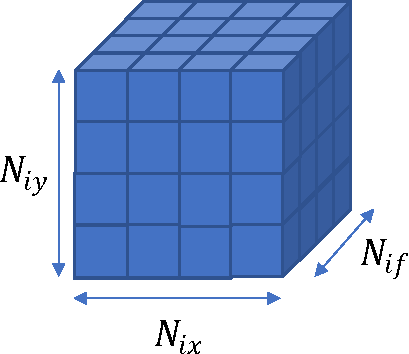
\includegraphics[width=\linewidth]{notifm.pdf}
    \caption{Input \acrshort{fm}}
    \label{fig:notation:ifm}
    \end{subfigure}
    %
    \begin{subfigure}[t]{.32\textwidth}
    \centering
    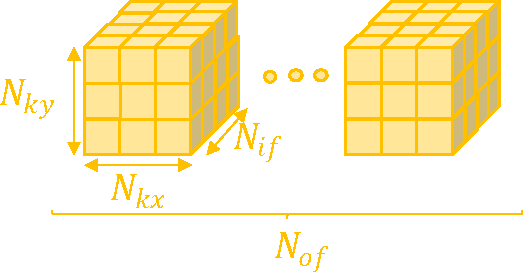
\includegraphics[width=\linewidth]{notk.pdf}
    \caption{A convolution kernel}
    \label{fig:notation:k}
    \end{subfigure}
    %
    \begin{subfigure}[t]{.32\textwidth}
    \centering
    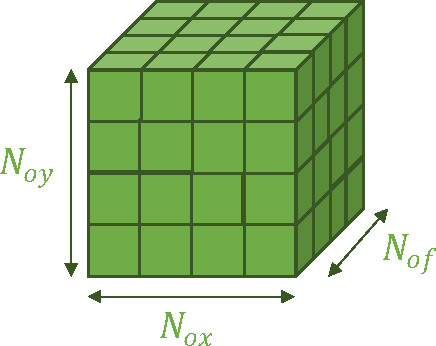
\includegraphics[width=\linewidth]{notofm.pdf}
    \caption{Output \acrshort{fm}}
    \label{fig:notation:ofm}
    \end{subfigure}
    %
    \caption{Volumes involved in the convolution operations}
    \label{fig:notconv}
\end{figure}
%
The convolution operation is illustrated in Figure \ref{fig:convolution}. It can be considered as a specialized linear operation and is divided in five steps \cite{matteucci_artificial_2019, zhu_efficient_2020}:
%
\begin{enumerate}
    \item A window of the same size than a kernel extracts a chunk of pixels from the input \acrshort{fm}.
    \item The extracted chunk of pixels is multiplied element-wise with a kernel.
    \item The ouput pixel is obtained by summing the products from previous step.
    \item The previous steps produce one output pixel of one channel. To compute one output channel, we simply slide the window on the input \acrshort{fm} and repeat the first three steps. The output pixel at position $(x, y)$ is obtained by the movement of the sliding window from the top left of the input \acrshort{fm}. 
    \item We repeat the previous operations with each kernel of the weight filter to obtain the output \acrshort{fm}.
\end{enumerate}
%
\begin{figure}[H]
    \centering
    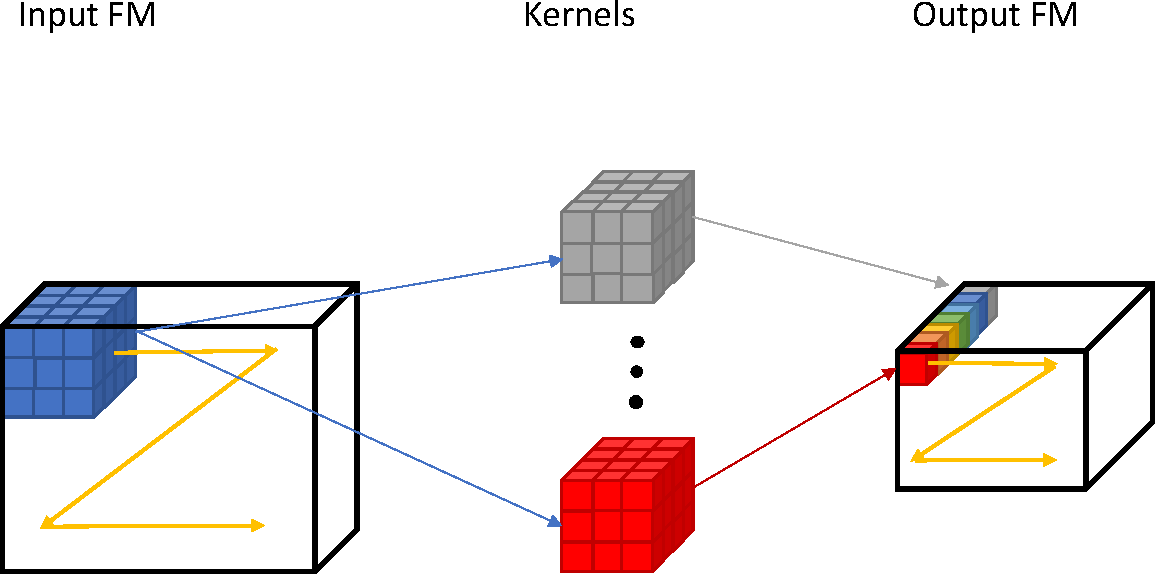
\includegraphics[width=\textwidth]{conv.pdf}
    \caption{Convolution operation}
    \label{fig:convolution}
\end{figure}
%
Except for $1 \times 1$ kernel, a spatial reduction between the input and output \acrshort{fm} is observed, while the convolution can be used to increase the number of channel (if $N_{if} < N_{of}$). It is explained by the fact that the sliding window movements can not go beyond the size of the input \acrshort{fm}. We can express the spatial reduction using equation \eqref{label:conv_spatial_red} \cite{ma_optimizing_2018}.
%
\begin{equation}
    N_{o\{x,y\}} = N_{i\{x,y\}} - N_{k\{x,y\}} + 1
    \label{label:conv_spatial_red}
\end{equation}
%
\textit{Padding} can be used on the edges in order avoid this spatial reduction. It consists of increasing the spatial dimensions (width and height) of the input \acrshort{fm} by insterting on the edges extra pixels (usually 0 value) \cite{liu_fpga-based_2019}. Using padding, the spatial dimension increase can be expressed using Equation \eqref{eq:pad-incr}, where $N_{i'\{x,y\}}$ are the spatial dimensions of the input \acrshort{fm} with padding applied. If we replace $N_{i\{x,y\}}$ by $N_{i'\{x,y\}}$ in Equation \eqref{label:conv_spatial_red}, there is no reduction in the dimensions.
%
\begin{equation}
    N_{i'\{x,y\}} = N_{i\{x,y\}} + N_{k\{x,y\}} - 1
    \label{eq:pad-incr}
\end{equation}

The sliding movement of the window on the input \acrshort{fm} is called the \textit{stride} and is initially set to 1. The stride can be increased to decrease the spatial dimensions of the output FM \cite{liu_fpga-based_2019}. For example, if a padding and a stride of 2 are used : $\frac{N_{ix}}{N_{ox}} = \frac{N_{iy}}{N_{oy}} = \frac{1}{2}$, and the output \acrshort{fm} has 4 times fewer pixels. Equation \eqref{label:conv_spatial_red_tot} represents the spatial reduction during convolution in function of the stride \cite{ma_optimizing_2018}. There are also other ways to reduce the spatial dimensions of the output \acrshort{fm}. One of them will be developed in the next section.
%
\begin{equation}
    N_{o\{x,y\}} = \left\lfloor \frac{ N_{i\{x,y\}}}{S} \right\rfloor - N_{k\{x,y\}} + 1
    \label{label:conv_spatial_red_tot}
\end{equation}

In summary, the whole convolution operation can be mathematically defined by Equation \eqref{eq:conv} \cite{abdelouahab_accelerating_2018}.
%
{\small
\begin{equation}
    \begin{split}
        \forall ox \in \{ 1, ..., N&_{ox} \}, oy \in \{ 1, ..., N_{oy} \}, of \in \{ 1, ..., N_{of} \}: \\
        FM_O[ox, oy, oc&] = \sum^{N_{if}}_{if=1}
        \sum^{N_{kx}}_{kx=1}
        \sum^{N_{ky}}_{ky=1}\\
        & FM_I \left[ ox \cdot S + kx - \left\lfloor \frac{N_{kx}}{2} \right\rfloor,  oy \cdot S + ky - \left\lfloor \frac{N_{ky}}{2} \right\rfloor, if \right] \cdot
        W^{of}_{if} \left[ kx, ky \right]
    \end{split}
    \label{eq:conv}
\end{equation}
}

According to \textcite{goodfellow_deep_2016}, the convolutional layer shows several advantages compared to the fully connected layer. Indeed, the convolutional layer is sparsely connected, which means that there are fewer connections between the different layers. The convolutional layer is then easier to train and the convolution keeps spatial information. 

Moreover, it has also parameter sharing: the same kernel is used to compute one channel of the output \acrshort{fm} and fewer parameters are needed. To illustrate this weight reduction, in AlexNet \cite{krizhevsky_imagenet_2012}, 94\% of the weights are used in the fully connected layers. But as said previously, convolution is a computationally heavy operation. For example, in VGG-11, 98.2\% of the operations are done in the convolution layers \cite{guo_survey_2018}. 

Furthermore, if the input \acrshort{fm} is a vector ($N_{ix} = N_{iy} = 1$), then it means that the convolution and the fully connected layer perform the same operation.

As the convolution has a huge arithmetic complexity, we see in the following section an alternate way to perform convolution while reducing its complexity.
